\begin{frame}
	\frametitle{Beacons en entornos universitarios}
			\block{\it Introducción}
				\begin{itemize}
					\item Posibilidades amplias para apps en entornos universitarios.
					\item Cada universidad intenta tener su propia aplicación siguiendo un patrón similar.
					\item Estas aplicaciones se centran en ofrecer servicios propios.
				\end{itemize}
			\endblock{}
\end{frame}

%------------------------------------------------------------------

\begin{frame}
	\frametitle{Beacons en entornos universitarios}
		\begin{columns}
			\begin{column}{0.6\textwidth}
				\block{\it Posibles casos de uso en entornos universitarios}
					\begin{itemize}
						\item Guía a través del campus de la universidad.
						\item Acceso al parking y recuento de número de plazas disponibles.
						\item Gestión de eventose información, entrada automática.
						\item Actividades interactivas por el campus, jornadas de acogida u otros eventos.
						\item Despacho del profesorado e información
					\end{itemize}
				\endblock{}
			\end{column}
			\begin{column}{0.4\textwidth}
				\vfill 
				\begin{center}
					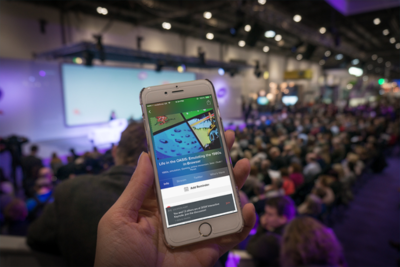
\includegraphics[width=0.9\linewidth]{Images/BeaconEvent}
				\end{center}
			\end{column}		
		\end{columns}
\end{frame}


%---------------------------------------------------------------------

\begin{frame}
	\frametitle{Beacons en entornos universitarios}
		\begin{columns}
			\begin{column}{0.6\textwidth}
				\block{\it Posibles casos de uso en entornos universitarios}
					\begin{itemize}
						\item Control de asistencia.
						\item Localizaciónde transporte público, horarios e informaciónde la parada.
						\item Biblioteca informativa.
						\item Control de acceso a instalaciones.
						\item Información y descuentos para usuarios de la app.
						\item Descarga automática de material.
					\end{itemize}
				\endblock{}
			\end{column}
			\begin{column}{0.4\textwidth}
				\vfill 
				\begin{center}
					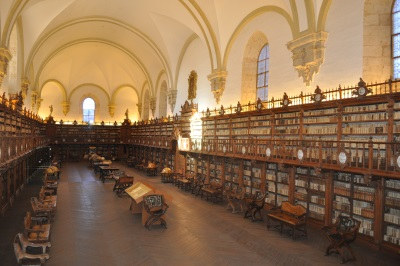
\includegraphics[width=0.9\linewidth]{Images/BibliotecaSalamanca}
				\end{center}
			\end{column}		
		\end{columns}
\end{frame}
